\documentclass{standalone}
\usepackage{tikz}

\begin{document}
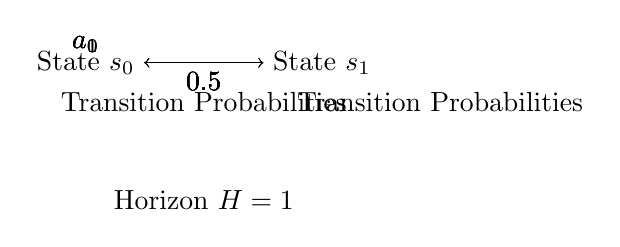
\begin{tikzpicture}[node distance=2cm]
    % Nodes
    \node (s0) at (0,0) {State $s_0$};
    \node (s1) at (3,0) {State $s_1$};

    % Edges with labels
    \draw[->] (s0) node[midway, above] {$a_0$} -- node[midway, below] {0.5} (s1);
    \draw[->] (s0) node[midway, above] {$a_1$} -- node[midway, below] {0.5} (s1);

    \draw[->] (s1) node[midway, above] {$a_0$} -- node[midway, below] {0.5} (s0);
    \draw[->] (s1) node[midway, above] {$a_1$} -- node[midway, below] {0.5} (s0);

    % Text for action probabilities
    \node at (1.5,-0.5) {Transition Probabilities};
    \node at (4.5,-0.5) {Transition Probabilities};

    % Horizon text
    \node at (1.5,-1.5) [below] {Horizon $H = 1$};
\end{tikzpicture}
\end{document}